\section{优化设计}

本章介绍了本文工作的具体设计。第一节给出AdaptiveLLM的整体设计方案, 后面的章节将分别介绍AdaptiveLLM中不同的功能模块。

\subsection{整体架构}

AdaptiveLLM实现了三个主要功能模块,包括张量重算分析器、张量交换分析器和自适应LLM推理加速器,其整体架构如图\ref{Fig:整体设计架构}所示。 \par

% 只有用户请求长度叫运行时信息,其他的不算,全文修改
其中, 张量重算分析器基于用户请求长度、模型隐藏维度、模型层数等信息来预测重算开销。张量交换分析器基于KV Cache内存占用和GPU-CPU双向传输带宽来预测交换开销。 自适应LLM推理加速器包含内存优化决策器和用户请求调度器。 内存优化决策器引入了基于开销感知的内存优化策略,提升总体吞吐率,实现面向服务器端的处理加速。 用户请求调度器引入了基于公平性的用户请求调度策略,减少单请求响应时间,实现面向客户端的实时处理。

\begin{figure}[!htbp]
  \centering
  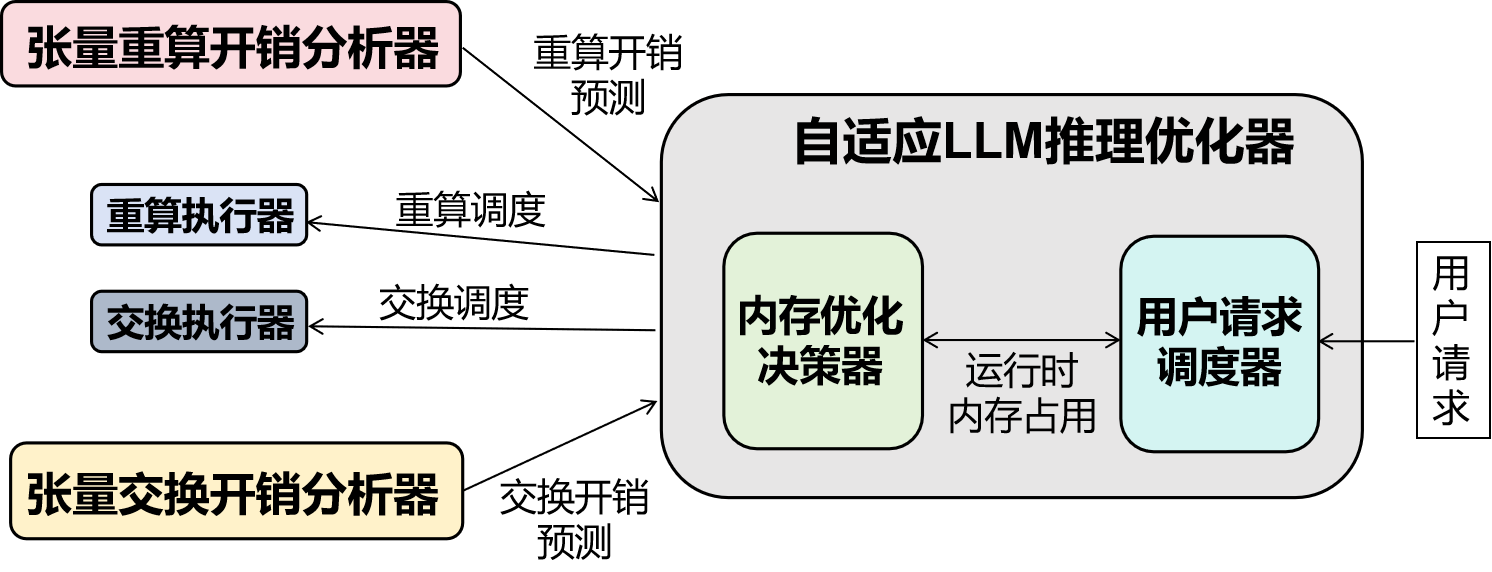
\includegraphics[width=0.9\linewidth]
  {整体设计架构.png}
  \caption{整体设计架构}
  \label{Fig:整体设计架构}
\end{figure}

在推理过程中,内存优化决策器与用户请求调度器共享运行时内存占用信息。在GPU内存不足时,内存优化决策器按照一定的算法选择优先级最低的用户请求进行抢占。其收集张量重算分析器提供的重算开销预测值与张量交换分析器提供的交换开销预测值,选择开销较小的抢占方式,而后交付相应的执行器。用户请求调度器在GPU内存空余时重新调度被抢占的用户请求,在满足公平性的前提下尽可能多地调度用户请求,避免GPU资源的浪费。二者高效协同,实现整体吞吐率与单请求延时的权衡。  \par

本章第二小节至第五小节将依次介绍张量重算分析器、张量交换分析器、内存优化决策器和用户请求调度器的设计原理与实现细节。

\subsection{张量重算分析器}

张量重算技术的时间线流程如图\ref{Fig:张量重算示意图}所示。当用户请求被抢占时,重算执行器在内存中删除其KV Cache;被重新调度时,执行一次prefill阶段来恢复被删除的数据。因此,张量重算引入的额外开销等于被抢占请求执行prefill阶段的时间。本文以OPT和Llama模型为例,通过算子粒复杂度分析来定位单步推理时间的影响因素。

\begin{figure}[!htbp]
  \centering
  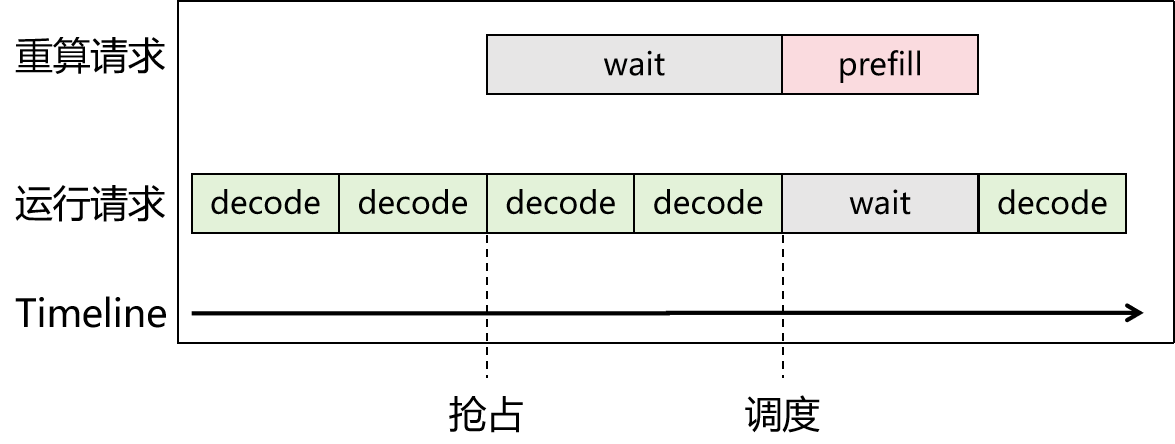
\includegraphics[width=0.9\linewidth]
  {张量重算示意图.png}
  \caption{张量重算时间线流程}
  \label{Fig:张量重算示意图}
\end{figure}

\subsubsection{算子粒度开销分析}

OPT和Llama模型中包含5种不同的算子:ReLU、Norm、Linear、SiluAndMul和Attention,其计算流程如图\ref{Fig:四种算子的计算流程}所示。图中$X_i$,$Y_i$是由用户输入决定的张量维度;$input\_dim$,$output\_dim$,$head\_size$是由算子决定的张量维度。 

\begin{figure}[!htbp]
  \centering
  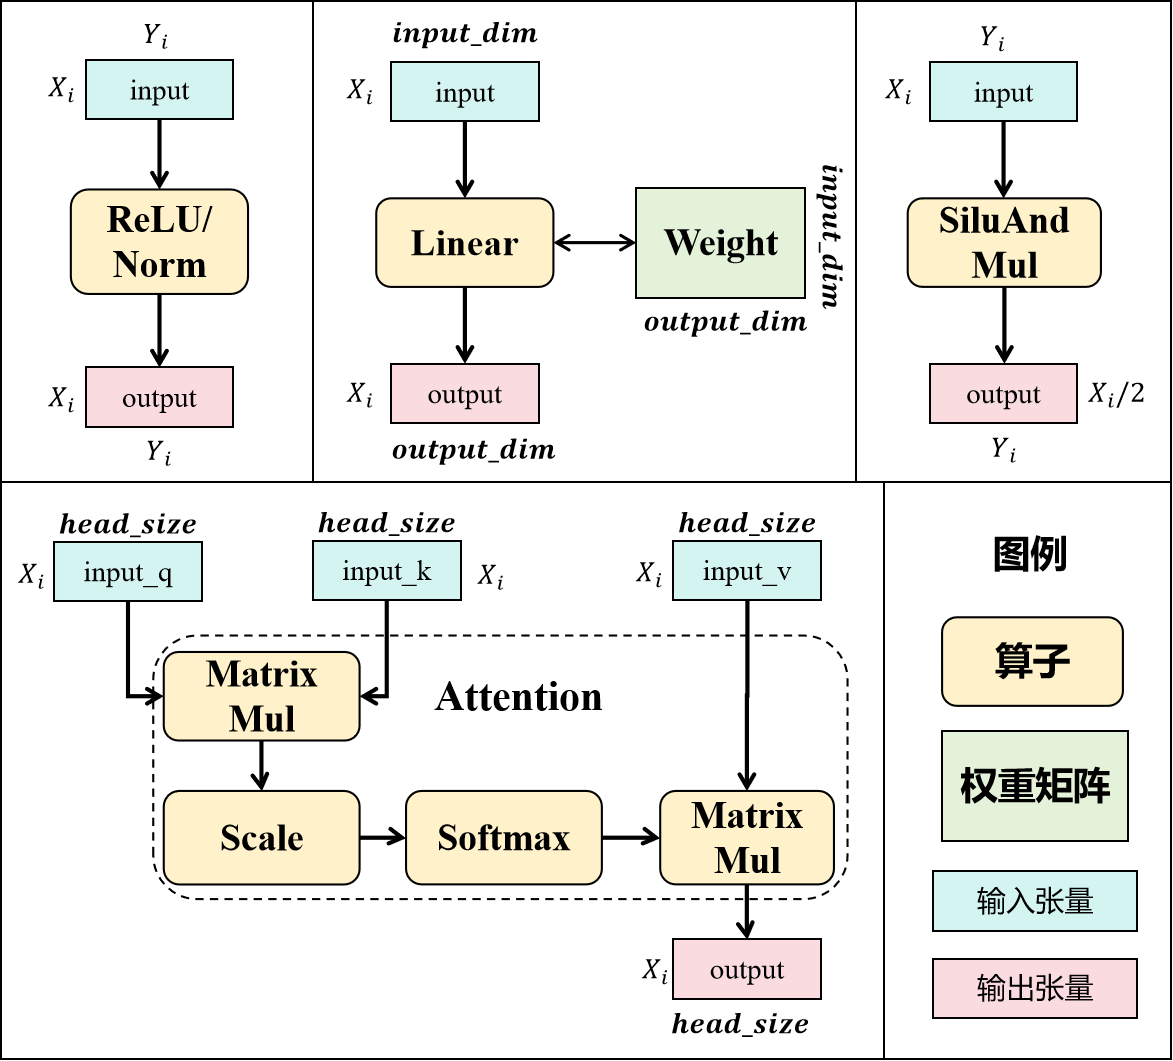
\includegraphics[width=0.9\linewidth]
  {四种算子的计算流程.png}
  \caption{四种算子的计算流程}
  \label{Fig:四种算子的计算流程}
\end{figure}

下面分别对这些算子进行复杂度分析。

\begin{itemize}
  \item \textbf{ReLU算子}:逐位调用激活函数进行计算,其时间复杂度为$O(X_i*Y_i)$。
  \item \textbf{Norm算子}:是LayerNorm、RMSNorm(仅在Llama模型中)等多种归一化算子的统称,其时间复杂度为$O(X_i*Y_i)$。
  \item \textbf{Linear算子}:是RowParallelLinear,ColumnParallelLinear等多种线性层的统称,将输入向量从$input\_dim$维空间映射到$output\_dim$维空间中,其计算复杂度为$O(X_i*input\_dim*output\_dim)$。
  \item \textbf{SiluAndMul算子}:该算子仅出现在Llama模型的MLP层中,将输入向量的指定维度减半,其时间复杂度为$O(X_i*Y_i)$。
  \item \textbf{Attention算子}:属于复合操作,由矩阵乘法、缩放和Softmax激活等底层算子组成,整体计算过程如公式\ref{Eq:Attention},其时间复杂度为$O(X_i^2*head\_size)$。
  \begin{equation}
    \small
    Attention(Q,K,V)=softmax(\frac{Q\times K^T}{\sqrt{h}}\times V)
    \label{Eq:Attention}
  \end{equation}
\end{itemize}
\par

根据算子粒度复杂度分析,可以找出4项有关LLM单步推理执行时间的影响因素,分别为:LLM层数、隐藏维度、单请求需要处理的token数量、和批处理大小。

\subsubsection{单步推理开销预测模型}

单步迭代执行时间预测是一项拥有4个输入变量,1个输出变量的回归预测任务。根据算子粒度时间复杂度分析可知,输出变量与输入变量之间存在多项式依赖关系。因此,本文共选用了9个回归模型,包括线性回归模型、支持向量机回归模型、决策树回归模型、随机森林回归模型、岭回归模型、套索回归模型、弹性回归模型、梯度提升回归模型、和K-临近回归模型。针对每种回归模型,对不同的多项式拟合次数(1到5)进行测试。选择在测试集上预测误差最小的配置,并将其部署到AdaptiveLLM的张量重算分析器中。 

\subsection{张量交换分析器}

张量交换的时间线流程如图\ref{Fig:张量交换示意图}所示。当用户请求被抢占时,交换执行器将其KV Cache从GPU中传输到CPU中(换出阶段);被重新调度时,将其KV Cache传输回GPU中(换入阶段)。因此,张量交换引入的额外开销等于换出时间与换入时间之和。\par

\begin{figure}[!htbp]
  \centering
  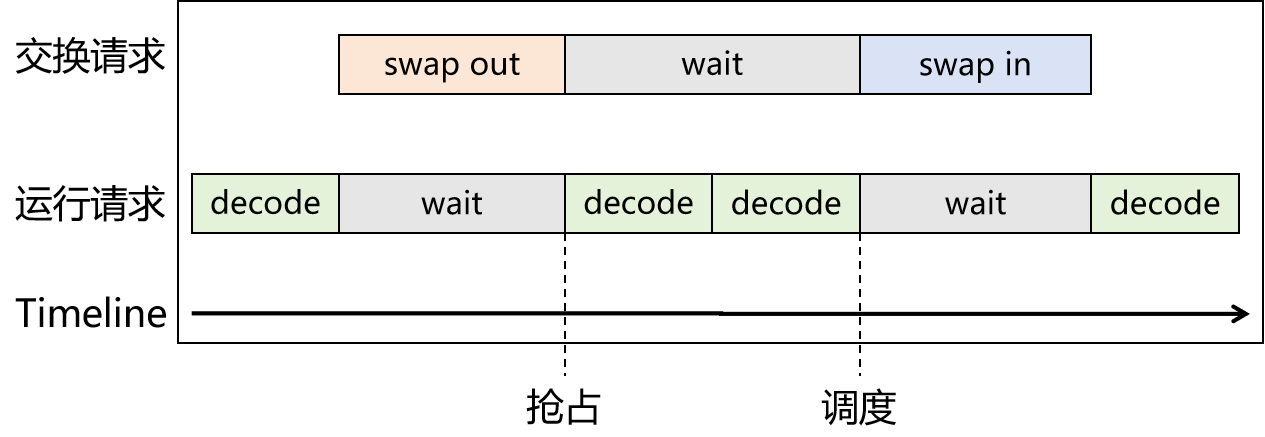
\includegraphics[width=0.9\linewidth]
  {张量交换示意图.png}
  \caption{张量交换时间线流程}
  \label{Fig:张量交换示意图}
\end{figure}

换出开销与换入开销的计算方式如公式\ref{Eq:Swap Overhead}所示。

\begin{equation}
  \begin{aligned}
    SwapOut\_Time=\frac{KVCache}{DtoH-bandwidth} \\
    SwapIn\_Time=\frac{KVCache}{HtoD-bandwidth}
  \end{aligned}
  \label{Eq:Swap Overhead}
  \setlength{\abovedisplayskip}{0ex}
  \setlength{\belowdisplayskip}{2ex}
\end{equation}

其中$DtoH-bandwidth$ 是GPU传输数据到CPU的带宽, $HtoD-bandwidth$是CPU传输数据到GPU的带宽。 AdaptiveLLM继承了vLLM所采用的Paged Attention技术,在GPU和CPU内存中划分大小固定的Block,用于存储KV Cache。每个Block内存占用的计算公式为\ref{Eq:Block Mem},其中$block\_size$是用户定义的参数,用于调整Block大小。

\begin{equation}
  \begin{aligned}
    block\_mem = num\_layers \times hidden\_size \times 
    \\ block\_size \times sizeof(float16)
  \end{aligned}
  \label{Eq:Block Mem}
  \setlength{\abovedisplayskip}{0ex}
  \setlength{\belowdisplayskip}{2ex}
\end{equation}

因此,假设一个用户请求的长度为$n$,占用GPU block的数量为$block\_num$,则其KV Cache占用的总内存空间为公式\ref{Eq:KV Cache Mem}。

\begin{equation}
  \begin{aligned}
    KVCache = 2 * block\_mem * block\_num  \\ =  2 * block\_mem * \lceil \frac{n}{block\_size} \rceil
  \end{aligned}
  \label{Eq:KV Cache Mem}
  \setlength{\abovedisplayskip}{0ex}
  \setlength{\belowdisplayskip}{2ex}
\end{equation}

由此可以计算出张量交换引入的额外开销。在上述公式中,换入换出传输带宽是由实验环境所决定的,在传输数据量较大时基本保持稳定。而$block\_size$与$block\_mem$在推理任务中均保持不变。因此对于不同的用户请求,其区别仅在于序列长度$n$的不同。

%wsq 抢占方式就是内存优化方式?是的话统一下用词
\subsection{内存优化决策器}

当GPU内存不足时,需要启动内存优化策略。AdaptiveLLM中的内存优化策略分为张量交换和张量重算两种。根据上文的分析,张量交换引入的额外开销等于KV Cache的换出开销与换入开销之和;张量重算引入的额外开销等于prefill过程的开销。\par

张量交换和张量重算所带来的额外开销成为了阻拦用户请求并发度进一步提升的瓶颈,因此抢占方式的选择尤为重要,在不同的运行环境中,应该使用不同的抢占策略来实现较低的抢占开销。然而,vLLM在抢占策略的选择上并未考虑开销问题,针对使用贪心采样策略的用户请求,其执行重算抢占;针对使用并行采样或束搜索采样策略的用户请求,其执行交换抢占。这种固定式抢占策略使得vLLM在面对GPU内存瓶颈时难以有效地压缩开销,进而无法提升吞吐率。本文则对两种抢占方式的开销进行比较,选择更优的抢占方式执行。内存优化决策器的工作流程如算法\ref{Code:内存优化决策器工作流程}所示。\par

当剩余的GPU内存空间不足以存放当前用户请求批次在下一个迭代中产生的KV Cache时(第2行),内存优化决策器进入工作状态。选择当前批次中优先级最低的用户请求(第3行),调用张量交换分析器和张量重算分析器来预测其交换和重算开销(第4、5行)。如果交换开销小于重算开销,则将该请求交付交换执行器处理(第7、8行);否则交付重算执行器处理(第10、11行)。以上过程循环执行,直至当前批次在下一个迭代中产生的KV Cache能够全部存放到GPU内存中。 

\begin{algorithm}
  \caption{Mem\_Schedule}
  \label{Code:内存优化决策器工作流程}
  \small
  \begin{spacing}{1.2}
    \begin{algorithmic}[1]
      \REQUIRE {运行队列$running$, 重算兼等待队列$waiting$, 交换队列$swapped$} 
      \ENSURE {无}
      \STATE {$sorted(running, key=<priority>, order=asc)$}
      \WHILE{$require\_mem(running) > available\_mem()$}
        \STATE {$req\gets running.pop()$}
        \STATE {$recomp\_time\gets GET\_RECOMP\_TIME(req)$}
        \STATE {$swap\_time\gets GET\_SWAP\_TIME(req)$}
        \IF {$swap\_time < recomp\_time$}
          \STATE {$SWAP(req)$} \hfill {// 交付张量交换执行器}
          \STATE {$swapped.append(req)$}
        \ELSE
          \STATE {$RECOMP(req)$} \hfill {// 交付张量重算执行器}
          \STATE {$waiting.append(req)$}
        \ENDIF
      \ENDWHILE
    \end{algorithmic}
  \end{spacing}
\end{algorithm}

%wsq 算两个开销前加个if判断,可以给个注释解释在干啥,如果内存不足直接选重算。两行完事儿?加一下吧
此外,当CPU内存不足时,内存优化决策器将直接调用张量重算,而跳过开销预测和比较过程。

\subsection{用户请求调度器}

本文维护三个用户请求队列:$waiting$队列、$running$队列与$swapped$队列。$waiting$队列存储初次进入调度系统,还未执行过,或者因张量重算而失去KV Cache的用户请求;$running$队列存储正在运行(执行decode阶段)的用户请求;$swapped$队列存储被换出到CPU中的用户请求。这三个队列之间拥有以下调度规则:

\begin{itemize}
  \item $running$队列中的用户请求运行完毕后会返回客户端,否则继续运行。
  \item 当GPU内存条件允许时,$swapped$队列中的用户请求可以直接转移至running队列中。
  \item 当GPU内存条件允许时,$waiting$队列中的用户请求可以转移至$running$队列中,但需要先执行prefill阶段。
\end{itemize}

如果剩余的GPU空间不足以存储$running$队列在下一次迭代中产生的KV Cache,则需要内存优化决策器进行抢占调度。如果剩余的GPU空间足够,则考虑扩充$running$队列,以避免浪费GPU资源。在扩充$running$队列时,用户请求调度器将部分请求从$swapped$队列或$waiting$队列中转移至$running$队列中。但由于两种转移方式存在较大差别(是否需要执行prefill阶段),因此每次扩充$running$队列时,或者仅从$swapped$队列进行调度,或者仅从$waiting$队列进行调度,而无法同时调度两个队列。用户请求调度器的工作流程如算法\ref{Code:用户请求调度器工作流程}所示。

\begin{algorithm}
  \caption{Req\_Schedule}
  \label{Code:用户请求调度器工作流程}
  \small
  \begin{spacing}{1.2}
    \begin{algorithmic}[1]
      \REQUIRE {大模型$LLM$}, {待执行的用户请求队列$L$}
      \ENSURE {无}
      \STATE {$w\gets L$}  \hfill {// 初始化waiting队列}
      \STATE {$r\gets empty\_list$} \hfill {// 初始化running队列}
      \STATE {$s\gets empty\_list$} \hfill {// 初始化swapped队列}
      \WHILE {$\neg (w.is\_empty()\land s.is\_empty() \land r.is\_empty())$}
        \STATE {$MemSchedule(r, w, s)$}  \hfill {// (内存不足时)抢占调度}
        \STATE {$s\_sche\gets SWAP\_IN\_SCHE()$}  \hfill {// 换入队列构建}
        \STATE {$w\_sche\gets RECOMP\_SCHE()$}  \hfill {// 重算队列构建}
        \IF {$GET\_PRI(w\_sche)\leq GET\_PRI(s\_sche)$}
          \STATE {$r=r+s\_sche$}  \hfill {// 换入调度}
          \STATE {$s=s-s\_sche$}
        \ELSE
          \STATE {$LLM.PREFILL(w\_sche)$}  \hfill {// 重算调度}
          \STATE {$r=r+w\_sche$}  
          \STATE {$w=w-w\_sche$}          
          \STATE \textbf{continue}
        \ENDIF
        \STATE {$LLM.DECODE(r)$} \hfill {// 单次推理迭代}
        \FOR {$req$ \textbf{in} $r$}
          \IF {$req.is\_finished()$}
            \STATE {$r.remove(req)$} \hfill {// 移除完成的请求}
          \ENDIF
        \ENDFOR
      \ENDWHILE
    \end{algorithmic}
  \end{spacing}
\end{algorithm}

客户端发送的用户请求进入$waiting$队列中,而$running$队列和$swapped$队列最初为空(第1-3行)。当GPU内存不足时,调用内存优化算法进行抢占调度(第5行),否则扩充$running$队列。 \par

用户请求调度器尽可能多地寻找能从$swapped$队列转移至$running$队列的用户请求(第6行),和能从$waiting$队列转移至$running$队列的用户请求(第7行)。对它们进行优先级比较(第8行),若前者的优先级均值较高,则将其直接转移到$running$队列中(第9-10行);若后者的优先级均值较高,则其执行prefill阶段后(第12行)转移至$running$队列中(第13-14行),同时直接进入下一轮迭代(第15行)。需要注意的是,当GPU内存不足时,无法实现从$swapped$队列或$waiting$队列向$running$队列的调度,即$w\_sche$和$s\_sche$队列均为空,此时也就不存在后续的优先级比较过程了。 \par

在以上调度操作完成后,$running$队列应当为非空的,否则推理过程无法继续。$running$队列执行decode阶段(第17行),将已完成的用户请求移除后进入下一次迭代(第18-22行)。 \par

对于一个用户请求,定义其优先级等于处理时间除以序列长度。其中,处理时间等于当前时刻减去该用户请求初次进入$waiting$队列的时刻,而序列长度为用户输入与已生成tokens的总长度。定义用户请求队列的优先级等于所有用户请求优先级的平均值。当用户请求初次进入$waiting$队列时,其序列长度较短,因此优先级增长较为迅速,能够被很快处理。而在用户请求等待过程中,其优先级在不断提升,因此避免了饥饿现象。 \par

% 这一段可以扔到实验分析里,分析为啥vllm差(如果后面实验部分没写的话),方法里不要写。
% vLLM基于FCFS策略进行设计,在调度时优先考虑$swapped$队列,只有当$swapped$队列为空时才调度$waiting$队列,使得以交换方式被抢占的用户请求相比于以重算方式被抢占的用户请求,其重调度的优先级更高。结合上一小节关于vLLM固定式抢占策略的分析可知,一部分用户请求被抢占后能够很快重新调度,而也有一部分用户请求被抢占后进入$waiting$队列的末位,需要长时间等待。这种调度策略违反了公平性原则。本文中的用户请求调度器基于公平性原则而设计,同时在实验部分证明,其能够大幅提升用户请求的实时性。